% Kryptologi: Hemmelig kommunikation
% Kryptografi: Sikring af indhold af kommunikation
% Steganografi: Usynliggørelse af kommunikationskanal
\subsection{Sikker kommunikation}
Der vil i dette afsnit blive kigget på hvad det vil sige at kommunikere sikkert, både i levering af kommunikationen, men også modtagelsen. 

\subsubsection{Kryptografi}
De fleste forbinder moderne IT-sikkerhed med højteknologiske krypteringsalgoritmer. Selvom dette er en vigtig del af IT-sikkerhed, er det dog ikke den eneste måde at sikre kommunikation på. Under emnet kryptologi, som omhandler alle former for hemmelig kommunikation, er kryptografi kun en del af emnet. Et andet vigtigt koncept som det dækker er steganografi, som vil blive diskuteret i næste afsnit. Den førnævnte algoritmebaseret sikring af data falder ind under kryptografi. Eksempler på disse spænder fra den simpleste alfabet skiftende, f.eks. én til højre, algoritme, til moderne hashing algoritmer. Fælles for anvendelsen af alle disse er dog, at det tydeligt viser en intention om at hemmeligholde indholdet. Hermed kan selve krypteringen gøre beskeden mistænkelig, da information af lav værdi ikke ville være besværet værd.

\subsubsection{Steganografi}
Som nævnt i indledningen, så består emnet kryptologi af flere underkategorier. Den kategori der vil blive fokuseret mest på her, er steganografi. Dette omhandler metoder til at skjule selve eksistensen af en given besked, i stedet for at gøre indeholdet ulæseligt, som er hvad kryptografi er.\cite{MeningOfSteganografi} Et eksempel på beskeder der er sikret med steganografi vil være de hemmelige signaler som der bruges af spioner i film. Et tilsyneladende tilfældigt symbol på et umiddelbart ligegyldigt sted, er blot en af de mange forskellige ting som kunne sende en besked sikkert frem. Alt dette vil foregå imens ingen andre vil opdage, at der overhoved var en form for kommunikation. Udenfor fiktion findes der også nogle eksempler på grupper som har udviklet systemer baseret på steganografi til at kommunikere internt.
\begin{figure}[H]
    \begin{subfigure}{0.5\textwidth}
    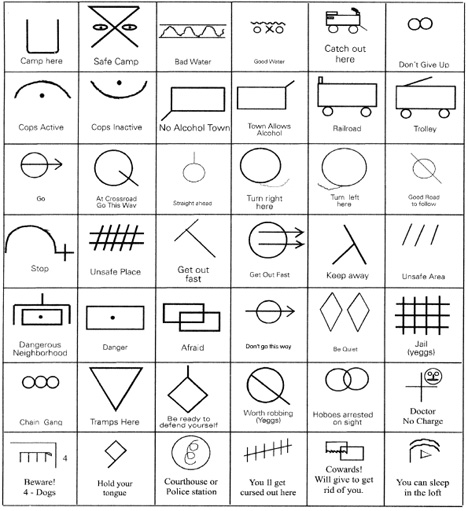
\includegraphics[width=0.9\linewidth, height=5cm]{Projectdoc/Problemanalyse/Illustrationer/hobo-glyphs-code.jpg} 
    \caption{The Hobo Code}
    \label{fig:hobocode}
    \end{subfigure}
    \begin{subfigure}{0.5\textwidth}
    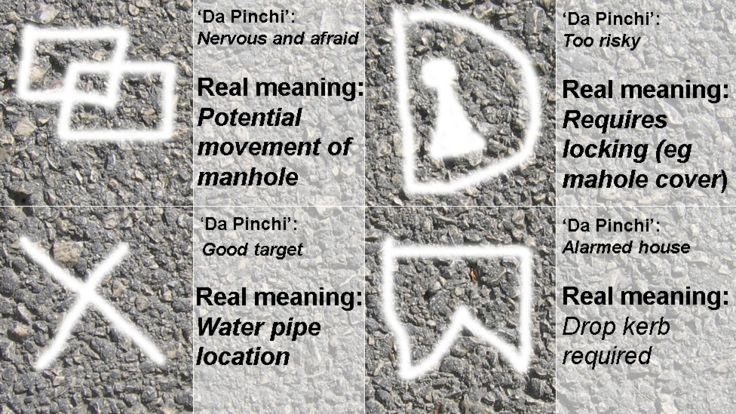
\includegraphics[width=0.9\linewidth, height=5cm]{Projectdoc/Problemanalyse/Illustrationer/BurglarsCode.jpg}
    \caption{Da Pinchi Code / The Burglars Code}
    \label{fig:burglarscode}
    \end{subfigure}
    \caption{To af de legendariske kryptografi metoder}
    \label{fig:legendscode}
\end{figure}
\noindent
Et kendt eksempel på en sådan steganografi metode kunne være "The Hobo Code [Se Figur: \ref{fig:hobocode}]", en bestemt del af kryptologien som er kendt, og anvendt, af hjemløse til at hjælpe hinanden med deres overlevelse\cite{TheHoboCode}. Disse beskeder er aldrig rigtigt blevet dateret, og ingen i dag kender derfor deres præcise oprindelse, men det vides dog stadig at denne kryptologiske metode har været anvendt i flere århundrede.\\ 
Foruden videnen om metodens eksistens gennem årene, vides også at der findes flere andre ligende afarter af denne kendte kode, såsom den nytidiske "Da Pinchi Code [Se Figur: \ref{fig:burglarscode}]". Denne kode bliver alment anvendt af konstruktions arbejdere, men siges også, efter historier, at have været anvendt af indbrudstyve eller andre kriminelle.\cite{DaPinchiCode}

% Ny titel
\subsubsection{Brugeren som sikkerhedsbrist}
I dag forsøger mange at bibeholde en, for dem værende, sikker eller hemmelig kommunikations mulighed. For nogle er disse muligheder dog mere sikre end hos andre. Som et eksempel vil de fleste private computerburgere, nok mene at deres generelle e-mail er forholdsvis sikker, men deres arbejdsplads deler muligvis ikke samme overbevisning. Dette var f.eks. tilfældet hos Hillary Clintons E-mail-skandale tilbage i 2015-2016. \cite{Hillary_Email_History} Hillary Clinton havde oprettet sin egen E-Mail server til håndtering af alle hendes mails, dog mener flere, blandet andet FBI, at denne aktion har været en "ekstremt uforsigtigt" håndtering af hendes fortrolighed. Trods Hillarys skandale menes dog ikke at et større sikkerhedsbrud har fundet sted, men Hillary har stadig som bruger mindsket den tilgængelige sikkerhed, i følge FBI, da de mener at hun fejlagtigt har misbrugt det vante system. \cite{Hillary_Email_skandale}

% Delkonklusion??? ny titel?
\subsubsection{Anvendelsen}
Dette faktum at der findes flere steganografiske metoder, der ikke er særligt kendte, som man stadig kan anvende uden at f.eks. politiet aner uråd, giver et indtryk af at man ville kunne anvende ligende metoder i en nyere teknologi og derved muligvis opnå samme effekt. \\
Man prøver i dag ved alle tænkelige metoder at kryptere forbindelser på nettet, hashe data og oplysninger, eller lige frem at danne sikre VPN tunler mellem sender og modtager. Men alle disse har det tilfældes med A-K koden og Morsing, at de er kendte og synlige, og derfor på et eller andet tidspunkt vil deres sikkerhed blive brudt. Men de legendariske steganografiske metoder har alle den vigtige egenskab at de færreste ligger mærke til dem, selvom de befinder sig lige foran dem, midt på den offentlige gade. Disse egenskaber kunne, muligvis ved nærmere studie, blive anvendt til videregivelse af beskeder på F.eks. De åbne sociale medier, så som Facebook, der allerede er kendt for at tilbageholde alle informationer til videregivelse eller studie. Ved andre tilfælde, kunne denne metode måske endda også anvendes til udveksling af information på tværs af modstående lande, så som Rusland og USA.

% Opsamling på hovedpointer igennem den første del.